\documentclass{standalone}
\usepackage{tikz}
\usetikzlibrary{patterns}
\usetikzlibrary{positioning}
\usetikzlibrary{patterns, positioning}
\usetikzlibrary{shapes.misc}
\usepackage[outline]{contour}
\contourlength{1.5pt} 
\usepackage[sfdefault]{ClearSans}

\begin{document}
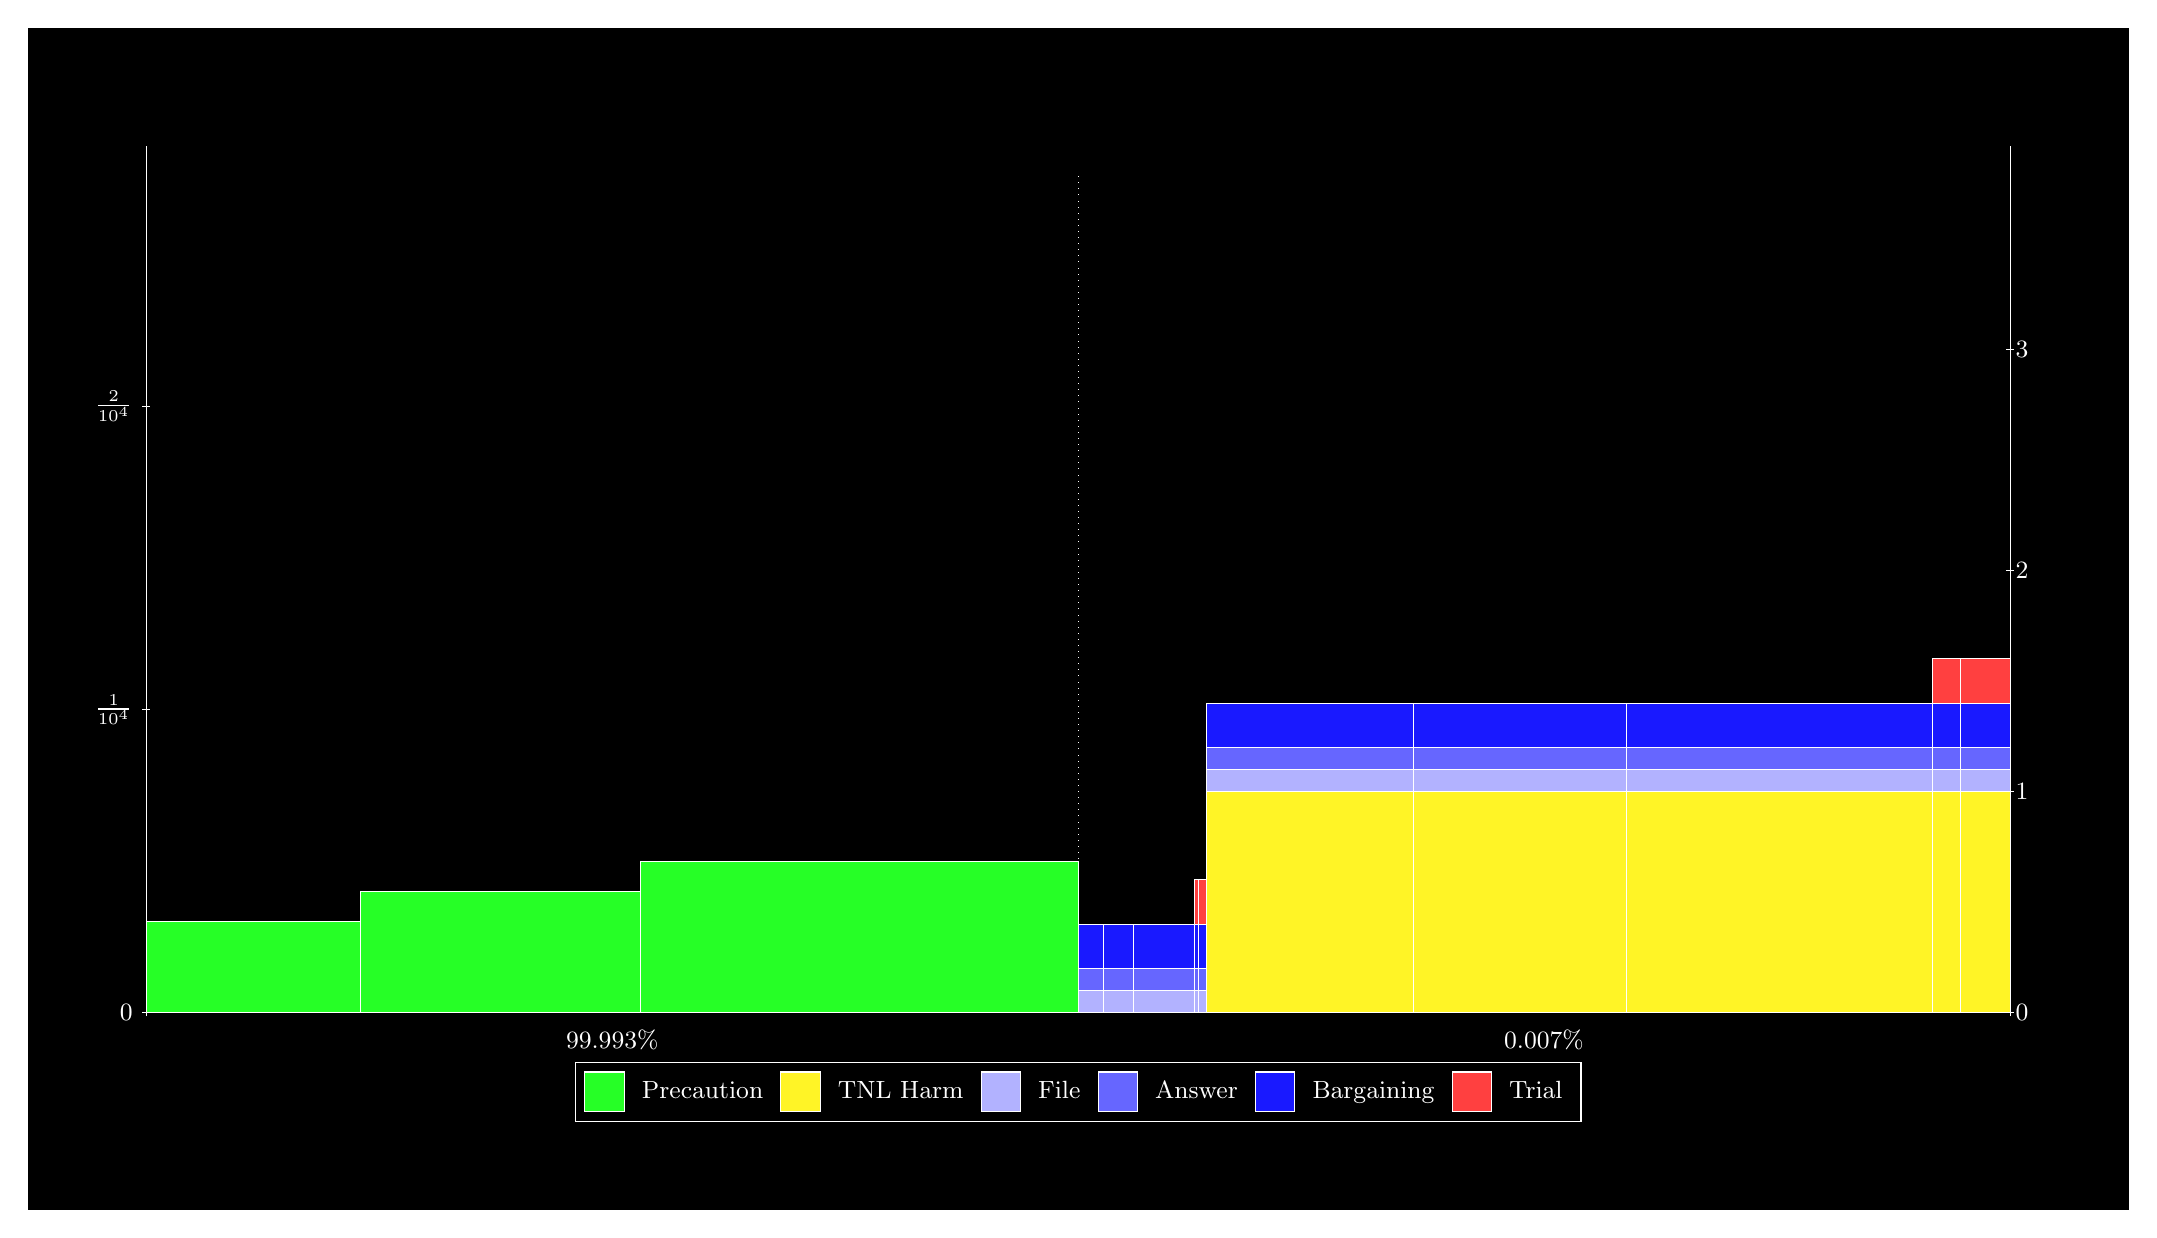
\begin{tikzpicture}
\draw[fill=black] (0,0) rectangle (26.667,15);
\draw[fill=green!85,draw=white,very thin] (1.5,2.5) rectangle (4.2218,3.6549);
\draw[fill=green!85,draw=white,very thin] (4.2218,2.5) rectangle (7.7721,4.0399);
\draw[fill=green!85,draw=white,very thin] (7.7721,2.5) rectangle (13.333,4.4248);
\draw[fill=green!85,draw=white,very thin] (13.333,2.5) rectangle (13.658,2.5001);
\draw[fill=blue!30,draw=white,very thin] (13.333,2.5001) rectangle (13.658,2.7809);
\draw[fill=blue!60,draw=white,very thin] (13.333,2.7809) rectangle (13.658,3.0618);
\draw[fill=blue!90,draw=white,very thin] (13.333,3.0618) rectangle (13.658,3.6235);
\draw[fill=green!85,draw=white,very thin] (13.658,2.5) rectangle (14.039,2.5001);
\draw[fill=blue!30,draw=white,very thin] (13.658,2.5001) rectangle (14.039,2.781);
\draw[fill=blue!60,draw=white,very thin] (13.658,2.781) rectangle (14.039,3.0618);
\draw[fill=blue!90,draw=white,very thin] (13.658,3.0618) rectangle (14.039,3.6236);
\draw[fill=green!85,draw=white,very thin] (14.039,2.5) rectangle (14.807,2.5001);
\draw[fill=blue!30,draw=white,very thin] (14.039,2.5001) rectangle (14.807,2.781);
\draw[fill=blue!60,draw=white,very thin] (14.039,2.781) rectangle (14.807,3.0619);
\draw[fill=blue!90,draw=white,very thin] (14.039,3.0619) rectangle (14.807,3.6236);
\draw[fill=green!85,draw=white,very thin] (14.807,2.5) rectangle (14.854,2.5001);
\draw[fill=blue!30,draw=white,very thin] (14.807,2.5001) rectangle (14.854,2.7809);
\draw[fill=blue!60,draw=white,very thin] (14.807,2.7809) rectangle (14.854,3.0618);
\draw[fill=blue!90,draw=white,very thin] (14.807,3.0618) rectangle (14.854,3.6235);
\draw[fill=red!75,draw=white,very thin] (14.807,3.6235) rectangle (14.854,4.1853);
\draw[fill=green!85,draw=white,very thin] (14.854,2.5) rectangle (14.958,2.5001);
\draw[fill=blue!30,draw=white,very thin] (14.854,2.5001) rectangle (14.958,2.781);
\draw[fill=blue!60,draw=white,very thin] (14.854,2.781) rectangle (14.958,3.0618);
\draw[fill=blue!90,draw=white,very thin] (14.854,3.0618) rectangle (14.958,3.6236);
\draw[fill=red!75,draw=white,very thin] (14.854,3.6236) rectangle (14.958,4.1853);
\draw[fill=green!85,draw=white,very thin] (14.958,2.5) rectangle (17.596,2.5001);
\draw[fill=yellow!85,draw=white,very thin] (14.958,2.5001) rectangle (17.596,5.3087);
\draw[fill=blue!30,draw=white,very thin] (14.958,5.3087) rectangle (17.596,5.5896);
\draw[fill=blue!60,draw=white,very thin] (14.958,5.5896) rectangle (17.596,5.8704);
\draw[fill=blue!90,draw=white,very thin] (14.958,5.8704) rectangle (17.596,6.4322);
\draw[fill=green!85,draw=white,very thin] (17.596,2.5) rectangle (20.301,2.5001);
\draw[fill=yellow!85,draw=white,very thin] (17.596,2.5001) rectangle (20.301,5.3087);
\draw[fill=blue!30,draw=white,very thin] (17.596,5.3087) rectangle (20.301,5.5896);
\draw[fill=blue!60,draw=white,very thin] (17.596,5.5896) rectangle (20.301,5.8705);
\draw[fill=blue!90,draw=white,very thin] (17.596,5.8705) rectangle (20.301,6.4322);
\draw[fill=green!85,draw=white,very thin] (20.301,2.5) rectangle (24.178,2.5001);
\draw[fill=yellow!85,draw=white,very thin] (20.301,2.5001) rectangle (24.178,5.3088);
\draw[fill=blue!30,draw=white,very thin] (20.301,5.3088) rectangle (24.178,5.5896);
\draw[fill=blue!60,draw=white,very thin] (20.301,5.5896) rectangle (24.178,5.8705);
\draw[fill=blue!90,draw=white,very thin] (20.301,5.8705) rectangle (24.178,6.4322);
\draw[fill=green!85,draw=white,very thin] (24.178,2.5) rectangle (24.531,2.5001);
\draw[fill=yellow!85,draw=white,very thin] (24.178,2.5001) rectangle (24.531,5.3087);
\draw[fill=blue!30,draw=white,very thin] (24.178,5.3087) rectangle (24.531,5.5896);
\draw[fill=blue!60,draw=white,very thin] (24.178,5.5896) rectangle (24.531,5.8704);
\draw[fill=blue!90,draw=white,very thin] (24.178,5.8704) rectangle (24.531,6.4322);
\draw[fill=red!75,draw=white,very thin] (24.178,6.4322) rectangle (24.531,6.9939);
\draw[fill=green!85,draw=white,very thin] (24.531,2.5) rectangle (25.167,2.5001);
\draw[fill=yellow!85,draw=white,very thin] (24.531,2.5001) rectangle (25.167,5.3087);
\draw[fill=blue!30,draw=white,very thin] (24.531,5.3087) rectangle (25.167,5.5896);
\draw[fill=blue!60,draw=white,very thin] (24.531,5.5896) rectangle (25.167,5.8705);
\draw[fill=blue!90,draw=white,very thin] (24.531,5.8705) rectangle (25.167,6.4322);
\draw[fill=red!75,draw=white,very thin] (24.531,6.4322) rectangle (25.167,6.9939);
\draw[white,very thin] (1.5,2.5) -- (1.5,13.5);
\draw[white,very thin] (1.45,2.5) -- (1.55,2.5);
\node[font=\small,text=white, anchor=east] at (1.45, 2.5) {0};
\draw[white,very thin] (1.45,6.3497) -- (1.55,6.3497);
\node[font=\small,text=white, anchor=east] at (1.45, 6.3497) {$\frac{1}{10^{4}}$};
\draw[white,very thin] (1.45,10.199) -- (1.55,10.199);
\node[font=\small,text=white, anchor=east] at (1.45, 10.199) {$\frac{2}{10^{4}}$};

\draw[white,dotted,very thin] (13.333,2.83) -- (13.333,13.17);
\draw[white,very thin] (25.167,2.5) -- (25.167,13.5);
\draw[white,very thin] (25.117,2.5) -- (25.217,2.5);
\node[font=\small,text=white, anchor=west] at (25.117, 2.5) {0};
\draw[white,very thin] (25.117,5.3086) -- (25.217,5.3086);
\node[font=\small,text=white, anchor=west] at (25.117, 5.3086) {1};
\draw[white,very thin] (25.117,8.1172) -- (25.217,8.1172);
\node[font=\small,text=white, anchor=west] at (25.117, 8.1172) {2};
\draw[white,very thin] (25.117,10.926) -- (25.217,10.926);
\node[font=\small,text=white, anchor=west] at (25.117, 10.926) {3};

\draw[white,very thin] (1.5,2.5) -- (25.167,2.5);
\draw[white,very thin] (1.5,2.45) -- (1.5,2.55);
\node[font=\small,text=white, anchor=north] at (1.5, 2.45) {};
\draw[white,very thin] (25.167,2.45) -- (25.167,2.55);
\node[font=\small,text=white, anchor=north] at (25.167, 2.45) {};

\node[font=\small,text=white,anchor=south] at (7.4167, 1.9) {99.993\%};
\node[font=\small,text=white,anchor=south] at (19.25, 1.9) {0.007\%};
\draw (13.3333,2.5) node (B) {};
\begin{scope}[align=center]
\matrix[scale=0.5,draw=white,below=0.5cm of B,nodes={draw},column sep=0.1cm]{
\node[rectangle,draw,minimum width=0.5cm,minimum height=0.5cm,fill=green!85]{}; & \node[draw=none,font=\small,text=white]{Precaution}; &
\node[rectangle,draw,minimum width=0.5cm,minimum height=0.5cm,fill=yellow!85]{}; & \node[draw=none,font=\small,text=white]{TNL Harm}; &
\node[rectangle,draw,minimum width=0.5cm,minimum height=0.5cm,fill=blue!30]{}; & \node[draw=none,font=\small,text=white]{File}; &
\node[rectangle,draw,minimum width=0.5cm,minimum height=0.5cm,fill=blue!60]{}; & \node[draw=none,font=\small,text=white]{Answer}; &
\node[rectangle,draw,minimum width=0.5cm,minimum height=0.5cm,fill=blue!90]{}; & \node[draw=none,font=\small,text=white]{Bargaining}; &
\node[rectangle,draw,minimum width=0.5cm,minimum height=0.5cm,fill=red!75]{}; & \node[draw=none,font=\small,text=white]{Trial}; \\\\
};\end{scope}

\end{tikzpicture}
\end{document}